
\chapter{ಏಪ್ರಿಲ್​ 10 ರಾಷ್ಟ್ರೀಯ ಭೂಮಾಪನಾ ದಿನಾಚರಣೆ}

ಲ್ಯಾಂಬ್​ಟನ್​ರವರು ತಮ್ಮ ಸರ್ವೇಯನ್ನು \enginline{1802} ಏಪ್ರಿಲ್​ \enginline{10} ರಂದು, ಮದ್ರಾಸಿನ ಕಡಲ ತೀರದ ಮೆರಿನಾ ಬೀಚ್​ನಿಂದ ಪ್ರಾರಂಭಿಸಿದರು. ಟ್ರಿಗನಮಿಟ್ರಿಕಲ್​ ಸರ್ವೇಯ ಟ್ರೈಯಾಂಗ್ಯುಲೇಷನ್​ ವಿಧಾನವದು. ಲ್ಯಾಂಬ್​ಟನ್​ರವರು ಪ್ರಾರಂಭಿಸಿದ ಬೇಸ್​ಲೈನಿನ ಒಂದು ತುದಿಯು, ಕಡಲ ತೀರದ ಸೇಂಟ್​ ಥಾಮಸ್​ ಮೌಂಟ್​. ಎರಡನೆಯ ತುದಿಯು ಇದರ ದಕ್ಷಿಣ ದಿಕ್ಕಿನ ಇನ್ನೊಂದು ಪರಂಬೋಕ್​ ಬೆಟ್ಟ. ಇವುಗಳ ನಡುವಿನ ಮಟ್ಟವಾದ ನೆಲದಲ್ಲಿ ಬೇಸ್​ಲೈನ್​ ಉದ್ದ \enginline{7.5} ಮೈಲು. ನೆಲವನ್ನು ನೇರ ಮಾಡಿ, ಸಮತಟ್ಟು ಮಾಡಿ, ನೂರಡಿಯ ಸ್ಟೀಲು ಚೈನನ್ನು ಬಿಡಿಸಿ, ಭಾರತೀಯ ಟ್ರಿಗನಮಿಟ್ರಿಕಲ್​ ಸರ್ವೇಯ ಮೊತ್ತ ಮೊದಲ ಬೇಸ್​ಲೈನಿನ ಅಳತೆಯ ಕಾರ್ಯವನ್ನು ಪ್ರಾಂಭಿಸಲಾಯಿತು. ಭಾರತದಲ್ಲಿ, ಕರ್ನಲ್​\break ಲ್ಯಾಂಬ್​ಟನ್​ರವರು ಕನಸುಕಂಡ ಮೊತ್ತಮೊದಲ ವೈಜ್ಞಾನಿಕ ಸರ್ವೇ ‘ದಿ ಗ್ರೇಟ್\break ​ ಟ್ರಿಗನಮಿಟ್ರಿಕಲ್​ ಸರ್ವೇ ಆಫ್​ ಇಂಡಿಯಾ’ ವನ್ನು ಆರಂಭಿಸಿದ ಶುಭ ದಿನವದು. ಈ ಸ್ಮರಣೀಯ ದಿನವನ್ನೇ ಪ್ರತಿ ವರ್ಷ ‘ರಾಷ್ಟ್ರೀಯ ಭೂಮಾಪನಾ ದಿನಾಚರಣೆ’ ಎಂದು ಎಲ್ಲಾ ರಾಜ್ಯಗಳ ಭೂಮಾಪನ ಇಲಾಖೆಯ ಆಶ್ರಯದಲ್ಲಿ, ಸರ್ವೇ ಆಫ್​ ಇಂಡಿಯಾದ ಆಶ್ರಯದಲ್ಲಿ, ದೇಶದೆಲ್ಲೆಡೆ ಸಡಗರದಿಂದ ಆಚರಿಸಿಕೊಂಡು ಬರಲಾಗುತ್ತಿದೆ.

ಏಪ್ರಿಲ್​ ಮೇ ಅವಧಿಯಲ್ಲಿ ಮದ್ರಾಸಿನ ತಾಪಮಾನ $80^\circ$ ಯಿಂದ $120^\circ$ ಫ್ಯಾರನ್​\break ಹೀಟ್​ ಇರುತ್ತದೆ. ಲ್ಯಾಂಬ್​ಟನ್​ರವರಿಗೆ ಬೆಂಕಿಯನ್ನೇ ಬಸಿಯುತ್ತಿರುವ ಈ ಉರಿಬಿಸಿಲಿನಲ್ಲಿಯೇ ನಡೆಸಬೇಕಾದ ಕೆಲಸದ ಬಗ್ಗೆ ಕಿಂಚಿತ್ತೂ ಚಿಂತೆಯಿರಲಿಲ್ಲ. ಚಿಂತೆ ಇದ್ದದ್ದು ಈ ಉರಿಬಿಸಿಲಿನಲ್ಲಿ, ಬಿಸಿಲಿನ ಸುಡು ತಾಪದಿಂದ ತಮ್ಮ ಸ್ಟೀಲ್​ ಚೈನಿನ ಉದ್ದವು ಹೆಚ್ಚು ಕಡಿಮೆ ಆಗಿ ಅದು ದೋಷಯುತವಾಗಿ ಬಿಡುತ್ತದೆ ಎಂದು. ಅನೇಕ ಪರೀಕ್ಷೆಗಳಿಂದ ಅವರು ಕಂಡುಕೊಂಡ ಅಂಶವೆಂದರೆ $1^\circ$ ಫ್ಯಾರನ್​ಹೀಟ್​ ಉಷ್ಣತೆಯ ಏರಿಕೆಯಿಂದ \enginline{100} ಅಡಿ ಉದ್ದದ ಚೈನ್​ನಲ್ಲಿ \enginline{0.0075} ಇಂಚಿನಷ್ಟು ಉದ್ದವು ವ್ಯತ್ಯಾಸವಾಗುತ್ತದೆ ಎಂದು. ಈ ಕಾರಣಕ್ಕೆ ಅಳತೆಯನ್ನು ಬೆಳಿಗ್ಗೆ ಮತ್ತು ಸಂಜೆಯ ತಂಪಾದ ಹೊತ್ತಿನಲ್ಲಿ ಮಾತ್ರ ಮಾಡಬೇಕಾಗಿತ್ತು. ಒಂದು ಇಂಚಿನ ಏಳು ಸಾವಿರದಲ್ಲಿ ಒಂದು ಭಾಗದಷ್ಟು ಕನಿಷ್ಠಾತಿ ಕನಿಷ್ಠ ಪ್ರಮಾಣದ ಅಳತೆಯ ವ್ಯತ್ಯಾಸವನ್ನು ಸಹ ಪರಿಗಣಿಸುವಷ್ಟು ಕೆಲಸದಲ್ಲಿ ನಿಖರತೆ, ಸೂಕ್ಷ್ಮತೆ, ತಾಳ್ಮೆ, ಸಹನೆ ಲ್ಯಾಂಬ್​ಟನ್​ರವರಿಗೆ. ಸಮಯವನ್ನು ಉಳಿಸಲು ಹೋಗಿ, ನಿಖರತೆಯನ್ನು ಎಂದೂ ತ್ಯಾಗ ಮಾಡಿದವರಲ್ಲ ಅವರು. ಸರ್ವೇಯ ಮುಖ್ಯ ಅವಶ್ಯಕತೆ ಎಂದರೆ ಅದು ನಿಖರತೆ. ಮ್ಯಾಪು ನಿಖರತೆಯ ಅವಶ್ಯಕತೆಯನ್ನು ಮೊದಲು ಪೂರೈಸುವಂತಿರಬೇಕು. ಮ್ಯಾಪಿನಲ್ಲಿ ನಿಖರತೆಯು ಅಂತರ್ನಿಹಿತ ಅಂಶವಾಗಿರಬೇಕು. ನಿಖರತೆಯಿಲ್ಲದ ಸರ್ವೇ ಅದು ಸರ್ವೇಯೇ ಅಲ್ಲ. ಲ್ಯಾಂಬಟನ್​ರವರ ಸರ್ವೇಯ ಮೂಲ ತತ್ವವೇ ಇದು. ಈ ಕೂದಲೆಳೆಯಷ್ಟು ನಿಖರತೆಯ ಬೇಸ್​ಲೈನ್​ ಅಳತೆ ಕಾರ್ಯಕ್ಕೆ ಅವರಿಗೆ ಒಟ್ಟು \enginline{57} ದಿನಗಳು ಹಿಡಿದವು.

ಟ್ರಿಗನಮಿಟ್ರಿಕಲ್​ ಸರ್ವೇಯಲ್ಲಿ, ಯಾವ ನಿಖರತೆಯಿಂದ ಬೇಸ್‌ಲೈನ್​ ಅಳತೆ ಕಾರ್ಯವನ್ನು ನಿರ್ವಹಿಸಲಾಗುವುದೋ ಅದೇ ನಿಖರತೆಯ ಮೇಲೆ ಇಡೀ ಟ್ರೈಯಾಂಗ್ಯುಲೇಷನ್​ ನಿಖರತೆಯು ನಿಂತಿರುತ್ತದೆ. ಬೇಸ್‌ಲೈನ್​ ಉದ್ದವು ಏನಿರಬೇಕೆಂದು, ಆ ಬೇಸ್‌ಲೈನನ್ನು ಆಧರಿಸಿ ನಿಂತಿರುವ ತ್ರಿಭುಜದ ಗಾತ್ರವು ಸೂಚಿಸುತ್ತದೆ. ಆದರೆ, ಸಂದರ್ಭ ಸನ್ನಿವೇಶ ಹೇಗಿರುತ್ತವೆಂದರೆ, ಕ್ಷೇತ್ರದಲ್ಲಿ \enginline{7} ರಿಂದ \enginline{8} ಮೈಲು ಮೀರಿದ ಬೇಸ್‌ಲೈನ್​ ಆಯ್ಕೆ ಅಸಾಧ್ಯವಾಗಿರುತ್ತದೆ. ಏಕೆಂದರೆ, ಬೇಸ್‌ಲೈನ್​ ಸಾಧ್ಯವಾದಷ್ಟೂ ಬಯಲು ಪ್ರದೇಶದಲ್ಲೇ ಇರಬೇಕು, ಸಮತಟ್ಟು ಪ್ರದೇಶದಲ್ಲೇ ಇರಬೇಕು. ಎರಡು ತುದಿಗಳು ಪರಸ್ಪರ ಗೋಚರಿಸಬೇಕು. ಅದರಿಂದ ರಚಿತವಾಗುವ ತ್ರಿಭುಜಗಳು ಸಮರೂಪಿ ತ್ರಿಭುಜಗಳಾಗಿರಬೇಕು.

ಭಾರತದಲ್ಲಿ ಮೊದಲಿಗೆ, ಲ್ಯಾಂಬ್​ಟನ್​ರವರ ಕಾಲದಲ್ಲಿ ಬೇಸ್‌ಲೈನ್​ ಅಳತೆಗೆ \enginline{100} ಅಡಿಯ ಸ್ಟೀಲು ಚೈನನ್ನು ಬಳಸಲಾಗುತ್ತಿತ್ತು. ಆದರೆ ಅನಂತರದಲ್ಲಿ, ಸ್ಟೀಲು ಚೈನ್​ ಬದಲಿಗೆ ಕಾಂಪನ್​ಸೇಷನ್​ ಬಾರ್​ನ್ನು ಬಳಸಲಾಯಿತು. ಇತರೆ ದೇಶಗಳಲ್ಲಿ ಪ್ಲಾಟಿನಮ್, ಕಾಪರ್​, ಕಬ್ಬಿಣದಿಂದ ಮಾಡಿದ ಲೋಹದ ರಾಡುಗಳನ್ನು ಸಹ ಬೇಸ್‌ಲೈನ್​ ಅಳತೆಗೆ ಬಳಸಲಾಗಿದೆ. ಸರಪಳಿಯನ್ನು ಅಥವಾ ಲೋಹದ ರಾಡನ್ನು ಬಳಸಿದಾಗ ಉಷ್ಣತೆಯ ಹಿಗ್ಗುವಿಕೆಗೆ ತಿದ್ದುಪಡಿಯನ್ನು ಅನ್ವಯಿಸಿಕೊಳ್ಳಬೇಕು. ಆದರೆ, ಕಾಂಪನ್​ಸೇಷನ್​ ಬಾರನ್ನು ಬಳಸಿದಾಗ ಉಷ್ಣತೆಗೆ ತಿದ್ದುಪಡಿಯ ಅವಶ್ಯಕತೆ ಇಲ್ಲ. ಏಕೆಂದರೆ, ಎಲ್ಲಾ ಉಷ್ಣತೆಯಲ್ಲೂ ಒಂದೇ ಉದ್ದವಿರುವಂತೆ ಕಾಂಪನ್​ಸೇಷನ್​ ಬಾರನ್ನು ವಿಶೇಷವಾಗಿ ರಚಿಸಲಾಗಿರುತ್ತದೆ.

ಈ ರೀತಿಯಾಗಿ ಬಹು ಎಚ್ಚರಿಕೆಯಿಂದ ಅಳೆದ ಬೇಸ್‌ಲೈನ್​, ತ್ರಿಭುಜದ ಸರಣಿಯ ಆರಂಭದ ಅಳತೆಯಾಗಿರುತ್ತದೆ. ಈ ತ್ರಿಭುಜೀಕರಣವು \enginline{150–200} ಮೈಲು ದೂರ ಕ್ರಮಿಸಿದಾಗ ಸೂಕ್ತ ಸ್ಥಳ ಸಿಕ್ಕಾಗ, ಲೆಕ್ಕಾಚಾರ ಮಾಡಿದ ಒಂದು ದೂರವನ್ನು ಪುನಃ ಇದೇ ಎಚ್ಚರಿಕೆ ನಿಖರತೆಯಿಂದ ಅಳೆಯಲಾಗುತ್ತದೆ. ಇದನ್ನು ವೆರಿಫಿಕೇಷನ್​ ಬೇಸ್‌ಲೈನ್​ ಎನ್ನುತ್ತಾರೆ. ಈ ವೆರಿಫಿಕೇಷನ್​ ಬೇಸ್‌ಲೈನ್​ ಅಳತೆಯಿಂದ ಇಡೀ ತ್ರಿಭುಜೀಕರಣದ ನಿಖರತೆಯನ್ನು ದೋಷವನ್ನು ಪರಿಶೀಲಿಸಬಹುದು ಮತ್ತು ಸರಿಪಡಿಸಿಕೊಳ್ಳಬಹುದು.

ಲ್ಯಾಂಬ್​ಟನ್​ರವರು ಮದ್ರಾಸಿನ ಕಡಲ ತೀರದ ಮೆರಿನಾ ಬೀಚ್​ನಿಂದ ಬೇಸ್‌ಲೈನ್​ ಅಳತೆ ಕಾರ್ಯ ಆರಂಭಿಸಿದ್ದರೂ ಬಹು ಮುಖ್ಯ ಉಪಕರಣವಾದ ಕ್ಯಾರಿ ಕಂಪನಿಯ, ಥಿಯಡೊಲೈಟ್​ ಉಪಕರಣವಿನ್ನೂ ಬಂದಿರಲಿಲ್ಲ. ಅದು ಇನ್ನೂ ಇಂಗ್ಲೆಂಡ್​ನಿಂದ ಹಡಗಿನಲ್ಲಿ ಬರಬೇಕಿತ್ತು. ಫ್ರೆಂಚ್​ ದೇಶದ ಕಾವಲುಪಡೆಯ ಹಡಗು ಈ ಥಿಯಡೊಲೈಟ್​ ಉಪಕರಣವನ್ನು ಹೊತ್ತು ತರುತ್ತಿದ್ದ ಹಡಗನ್ನು, ಯಾವುದೋ ಶತ್ರು ಪಡೆಯ ಮಿಲಿಟರೀ ಹಡಗು ಇರಬೇಕೆಂದು ಭಾವಿಸಿ, ವಶಪಡಿಸಿಕೊಂಡುಬಿಟ್ಟಿತ್ತು.

ಫ್ರೆಂಚ್​ನವರು, ಬ್ರಿಟೀಷ್​ನವರು ಆ ಕಾಲದ ಜಾಗತಿಕವಾದ ದೊಡ್ಡ ಶಕ್ತ ರಾಷ್ರಗಳು ಮತ್ತು ವಿರೋಧಿಗಳು. ವಶಪಡಿಸಿಕೊಂಡ ಈ ಹಡಗನ್ನು ಫ್ರೆಂಚ್​ನವರು ಮಾರಿಷಿಯಸ್​ ದ್ವೀಪಕ್ಕೆ ತೆಗೆದುಕೊಂಡು ಹೋದರು. ಅಲ್ಲಿ ಉಪಕರಣ ಇದ್ದ ಪೆಟ್ಟಿಗೆಯನ್ನು ಹಡಗಿನಿಂದ ಇಳಿಸಿ ತೆಗೆದು ನೋಡಿದರು. ಅದು ಸರ್ವೇ ಉಪಕರಣ. ಇಂಡಿಯನ್​ ಟ್ರಿಗನಮಿಟ್ರಿಕಲ್​ ಸರ್ವೇ ಕಾರ್ಯಕ್ಕೆ ಮುಖ್ಯವಾಗಿ ಬೇಕಾದ ಥಿಯಡೋಲೈಟ್​ ಉಪಕರಣ ಅದು. ಇದರ ಬರುವಿಕೆಗಾಗಿ ಮದ್ರಾಸಿನಲ್ಲಿ ಲ್ಯಾಂಬ್​ಟನ್​ರವರು ಕಾಯುತ್ತಿದ್ದರು. ಈ ಶ್ರೇಷ್ಠ ಕಾರ್ಯಕ್ಕಾಗಿ ಥಿಯಡೋಲೈಟ್​ ಅಲ್ಲಿಗೆ ಹಡಗಿನಲ್ಲಿ ತೆರಳುತ್ತಿದೆ ಎಂದು ಫ್ರೆಂಚರಿಗೆ ಅರಿವಾಯಿತು. ಅವರೂ ಕೂಡ ಈ ವೈಜ್ಞಾನಿಕ ಕಾರ್ಯಕ್ಕೆ ಸ್ಪಂದಿಸಿದರು. ಉಪಕರಣವನ್ನು ರೀಪ್ಯಾಕ್​ ಮಾಡಿ, ಮದ್ರಾಸ್​ ಸರ್ಕಾರಕ್ಕೆ ಅಭಿನಂದನಾ ಪತ್ರವನ್ನು ಬರೆದು, ಭಾರತಕ್ಕೆ ಗೌರವಯುತವಾಗಿ ಮರಳಿಸಿದರು. ಥಿಯಡೊಲೈಟ್​ ಉಪಕರಣವು, \enginline{1802}ರ ಸೆಪ್ಟಂಬರ್​ ವೇಳೆಗೆ ಮದ್ರಾಸ್​ ತಲುಪಿತು. ಆಗಿನ ಕಾಲದಲ್ಲಿ ತುಂಬಾ ಅಪರೂಪದ, ಇಡೀ ವಿಶ್ವದಲ್ಲಿಯೇ ಈ ಮಾದರಿಯ ಒಂದೊ ಎರಡೊ ಅಷ್ಟೇ ತಯಾರಾದ ವಿರಳ ಉಪಕರಣವದು.

ಥಿಯಡೊಲೈಟ್​ ಉಪಕರಣ ಎಂದರೆ, ಅದು ಮುಖ್ಯವಾಗಿ ಟೆಲಿಸ್ಕೋಪ್​ ಮತ್ತು ಕೋನಮಾಪಕಗಳ ಜೋಡಿ. ಟೆಲಿಸ್ಕೋಪ್​, ದೂರದ ಗುರುತೊಂದನ್ನು ವೀಕ್ಷಿಸಲು ಕ್ಷಿತಿಜೀಯ ಸಮತಲದಲ್ಲೂ, ಲಂಬ ಸಮತಲದಲ್ಲೂ ತಿರುಗುತ್ತದೆ. ಅಂದರೆ, ದೂರದ ಸ್ಟೇಷನ್​ ವೀಕ್ಷಿಸಲು ಟೆಲಿಸ್ಕೋಪನ್ನು ಕ್ಷಿತಿಜೀಯ ಸಮತಲದಲ್ಲಿರುವ ವರ್ತುಲಾಕಾರದ ಕೋನಮಾಪಕದ ತಟ್ಟೆಯ ಮೇಲೆ ಎಡಕ್ಕೂ ಬಲಕ್ಕೂ ತಿರುಗಿಸಿದಾಗ, ಸಮತಲ ಕೋನವು ಎಷ್ಟೆಂದು ದೊರೆಯುತ್ತದೆ. ಲಂಬ ಸಮತಲದಲ್ಲಿರುವ ಮತ್ತೊಂದು ವರ್ತುಲಾಕಾರದ ಕೋನಮಾಪಕದ ತಟ್ಟೆಯ ಮೇಲೆ, ಟೆಲಿಸ್ಕೋಪನ್ನು ಮೇಲಕ್ಕೂ ಕೆಳಕ್ಕೂ ಚಲಿಸಿದಾಗ, ಲಂಬ ಸಮತಲ ಕೋನವು ಎಷ್ಟೆಂದು ದೊರೆಯುತ್ತದೆ. ಕ್ಷಿತಿಜೀಯ ಸಮತಲದಲ್ಲಿರುವ ವರ್ತುಲಾಕಾರದ, ಕೋನಮಾಪಕದ ತಟ್ಟೆಯ ವ್ಯಾಸವು \enginline{3} ಅಡಿ ಅಗಲ. ಈ ವರ್ತುಲಾಕಾರದ, ಕೋನಮಾಪಕದ ತಟ್ಟೆಯನ್ನು ಡಿಗ್ರಿ, ಮಿನಿಟ್​, ಸೆಕೆಂಡ್​ಗೆ ಓದುವ ವ್ಯವಸ್ಥೆ ಇರುವುದರಿಂದ, ಹಾರಿಜಾಂಟಲ್​ ಕೋನ ಮತ್ತು ವರ್ಟಿಕಲ್​ ಕೋನಗಳನ್ನು ಡಿಗ್ರಿ, ಮಿನಿಟ್​, ಸೆಕೆಂಡ್​ ನಿಖರತೆಗೆ ಅಳೆಯುವ ಅನುಕೂಲ ಇರುತ್ತದೆ. ಈ ಉಪಕರಣದ ಭಾರವು ಅರ್ಧ ಟನ್​. ಕಬ್ಬಿಣ ಹಿತ್ತಾಳೆಯಿಂದ ಮಾಡಿದ್ದು. ನಟ್ಟು ಬೋಲ್ಟ್​ಗಳನ್ನು ಬಿಚ್ಚಿ, ಬಿಡಿ ಭಾಗಗಳನ್ನು ಬೇರ್ಪಡಿಸಿ ಸಾಗಿಸಬೇಕು. ಇದನ್ನು ಹೊರಲು ಕಟ್ಟುಮಸ್ತಾದ ಒಂದು ಡಜನ್​ ಜನ ಬೇಕಾಗಿತ್ತು. ಎತ್ತಿನ ಗಾಡಿಯನ್ನು ಈ ಉಪಕರಣ ಸಾಗಿಸಲು ಬಳಸುವಂತಿರಲಿಲ್ಲ. ಏಕೆಂದರೆ ಎತ್ತಿನಗಾಡಿಯಲ್ಲಿ ಸಾಗಿಸಬೇಕೆಂದರೆ, ಅಲ್ಲಿ ರಸ್ತೆ ಇರಬೇಕು. ಸರ್ವೇ ತಾಣಕ್ಕೆ ಹೆಚ್ಚಿನ ಸಂದರ್ಭದಲ್ಲಿ ರಸ್ತೆ ಇರುವುದಿಲ್ಲ. ರಸ್ತೆ ಇದ್ದರೂ ಸಹ, ರಸ್ತೆಯಲ್ಲಿ ಗಾಡಿಯ ಕುಲುಕಾಟ ಇರುತ್ತದೆ. ಈ ಕುಲುಕಾಟದಿಂದ ಉಪಕರಣಕ್ಕೆ ಹಾನಿಯಾಗುತ್ತದೆ. ಆದ್ದರಿಂದ, ಎತ್ತಿನ ಗಾಡಿಯನ್ನು ಈ ಉಪಕರಣ ಸಾಗಿಸಲು ಬಳಸುವಂತಿರಲಿಲ್ಲ.

\begin{figure}[!htbp]
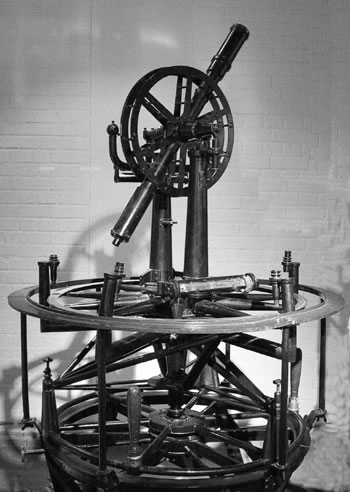
\includegraphics{"images/image007.jpg"}
\caption{ಟ್ರಿಗನಮಿಟ್ರಿಕಲ್​ ಸರ್ವೇ ಕಾರ್ಯಕ್ಕೆ ಬಳಸಿದ ಥಿಯಡೊಲೈಟ್​ ಉಪಕರಣ}\label{chap5-fig1}
\end{figure}

ಸೆಪ್ಟಂಬರ್​ ಕೊನೆಯ ಭಾಗದಲ್ಲಿ ಲ್ಯಾಂಬ್​ಟನ್​ರವರು ಬೇಸ್‌ಲೈನ್​ನ ಎರಡು ತುದಿಗಳಿಂದಲೂ ಪೂರ್ವ ನಿಗಧಿತ ಪಶ್ಚಿಮ ದಿಕ್ಕಿನ \enginline{3}ನೇ ಬಿಂದುವಿಗೆ ತಮ್ಮ ಗ್ರೇಟ್​ ಥಿಯಡೊಲೈಟ್​\break ನಿಂದ ಕೋನವನ್ನು ಓದಿದರು. ಆರಂಭದ ಬಿಂದುವಿನಲ್ಲಿ ಖಗೋಳ ವೀಕ್ಷಣೆ ಮಾಡಿ, ಅಕ್ಷಾಂಶ, ರೇಖಾಂಶಗಳ ಮೌಲ್ಯವನ್ನು ಕಂಡುಹಿಡಿದು, ಅದರ ಜಾಗತಿಕ ಸ್ಥಾನವನ್ನು ನಿಗಧಿ ಮಾಡಿದರು. ಅದರ ಸರಾಸರಿ ಸಮುದ್ರ ಮಟ್ಟವನ್ನು ಸಹ, ಪಕ್ಕದಲ್ಲಿಯೇ ಇರುವ ಸಮುದ್ರದಿಂದ ಒಯ್ದು ಗೊತ್ತುಪಡಿಸಿದರು. ಈಗ, ಮದ್ರಾಸಿನ ಬೇಸ್‌ಲೈನ್​ನ ಸ್ಥಾನವು, ಮೂರು ಆಯಾಮದಲ್ಲಿ, ಜಾಗತಿಕವಾಗಿ ಏನು ಎಂದು ನಿರ್ಧಾರಿತವಾಯಿತು. ಈ ಬೇಸ್‌ಲೈನನ್ನು ಆಧರಿಸಿ, ಅಕ್ಕ ಪಕ್ಕದ ವಿಶಾಲ ಪ್ರದೇಶದಲ್ಲಿ ಮುಂದುವರೆದು ರಚಿತವಾಗುವ ಟ್ರೈಯಾಂಗ್ಯುಲೇಶನ್​ ಸ್ಟೇಷನ್​ಗಳ ಸ್ಥಾನಗಳೂ ಸಹ ಈ ಬೇಸ್‌ಲೈನ್​ ಬಿಂದುಗಳಿಗೆ ಅನುಗುಣವಾದ ದೂರ, ದಿಕ್ಕು, ಎತ್ತರಗಳಲ್ಲಿ ನಿರ್ಧರಿತವಾಗುತ್ತವೆ. ನಿಂತ ಸ್ಥಾನದ ಭೌಗೋಳಿಕ ಅಕ್ಷಾಂಶ, ರೇಖಾಂಶ, ಸರಾಸರಿ ಸಮುದ್ರ ಮಟ್ಟದಿಂದ ಅದರ ಎತ್ತರ ಇವು ತಿಳಿದಿದ್ದರೆ, ವೀಕ್ಷಣೆ ಮಾಡಿದ ಬಿಂದುವಿನ ಭೌಗೋಳಿಕ\break ಮೌಲ್ಯವನ್ನೂ ಸಹ ನಿಖರವಾಗಿ ಲೆಕ್ಕಾಚಾರ ಮಾಡಬಹುದು. ಹೀಗೆ ಯಾವುದೇ ಪರ್ವತದ ಶಿಖರದ ಎತ್ತರವನ್ನೂ, ಅದರ ಸ್ಥಾನವನ್ನು ನಿಖರವಾಗಿ ಮ್ಯಾಪು ಮಾಡಬಹುದು. ಹಾಗು ಸರಾಸರಿ ಸಮುದ್ರ ಮಟ್ಟದಿಂದ ಅದರ ಎತ್ತರವನ್ನು ತಿಳಿಯಬಹುದು

ಒಂದು ಕೋನವನ್ನು, ದಿನದ ಕನಿಷ್ಟ ನಾಲ್ಕು ಬೇರೆ ಬೇರೆ ಅವಧಿಯಲ್ಲಿ, ಬೆಳಿಗ್ಗೆ ಸಾಯಂಕಾಲ ಅಳೆಯಬೇಕು. ಪ್ರತಿಸಲ ಥಿಯಡೋಲೈಟ್​ನ ಮುಖ ಬದಲಾವಣೆ ಮಾಡಬೇಕು. ಕೋನಮಾಪಕದ ಬೇರೆ ಬೇರೆ ಕ್ವಾಡ್ರಂಟ್​ಗಳಲ್ಲಿ ಕೋನ ವೀಕ್ಷಣೆ ಮಾಡಬೇಕು. ಈ ಎಲ್ಲಾ ಅಳತೆಯ ಸರಾಸರಿ ತೆಗೆದುಕೊಂಡರೆ ಉಪಕರಣದಲ್ಲಿನ ದೋಷವನ್ನು ನಿವಾರಣೆ ಮಾಡಿದಂತಾಗುತ್ತದೆ. ಟ್ರೈಯಾಂಗ್ಯುಲೇಷನ್​ ಕಾರ್ಯದಲ್ಲಿ ತ್ರಿಭುಜದ ಮೂರು ಕೋನಗಳನ್ನು ಅಳತೆ ಮಾಡುವುದನ್ನು ಲ್ಯಾಂಬ್​ಟನ್​ರವರು ಒತ್ತಿ ಹೇಳುತ್ತಿದ್ದರು. ತ್ರಿಭುಜದಲ್ಲಿ ಎರಡು ಕೋನವನ್ನು ಅಳೆದರೆ, ಮೂರನೇ ಕೋನವನ್ನು ಅಳೆಯದೆ, ಲೆಕ್ಕಾಚಾರದಿಂದ ಕಂಡುಕೊಳ್ಳಬಹುದು. ಆದರೆ ಟ್ರೈಯಾಂಗ್ಯುಲೇಷನ್​ ಕಾರ್ಯದಲ್ಲಿ ಪ್ರತಿ ಕೋನವನ್ನು ಅಳೆಯಲಾಗುತ್ತದೆ. ಸ್ಪೆರಿಕಲ್​ ಎಕ್ಸೆಸ್​ ತಿದ್ದುಪಡಿಯನ್ನು ಅನ್ವಯಿಸಲಾಗುತ್ತದೆ. ನಂತರ \enginline{3} ಕೋನಗಳನ್ನು ಕೂಡಿ, ಗಣಿತಾತ್ಮಕವಾಗಿ ತ್ರಿಭುಜದ \enginline{3} ಕೋನಗಳ ಮೊತ್ತ $180^\circ$ ಗೆ ತಾಳೆ ಇದೆಯಾ ಎಂದು ನೋಡಲಾಗುತ್ತದೆ. ಯಾವುದೇ ರೀತಿಯಲ್ಲೂ ದೋಷವಾಗದ ಹಾಗೆ ಪ್ರತಿ ಹೆಜ್ಜೆಯಲ್ಲೂ ಎಚ್ಚರಿಕೆ ವಹಿಸಲಾಗುತ್ತದೆ. ಒಂದೊಂದು ಕೋನವನ್ನು ಪುನಃ ಓದುವುದೆಂದರೆ ಪುನಃ \enginline{40–50} ಮೈಲುಗಳ ಕಾಡಿನ ನಡಿಗೆ. ಆಮೇಲೆ ಕೋನ ಓದಲು ಸೂಕ್ತ ಹವೆಯ ಸಮಯಕ್ಕೆ ಕಾಯುವುದು. ಇಷ್ಟೆಲ್ಲಾ ಎಚ್ಚರಿಕೆಯು ಸಣ್ಣ ಒಂದು ಡಿಗ್ರಿಯ ಒಂದು ಮಿನಿಟ್​ನ ಒಂದು ಸೆಕೆಂಡಿನ ಅಲ್ಪಾತಿ ಅಲ್ಪ ಭಾಗಾಂಶ ಪ್ರಮಾಣದ ನಿಖರತೆಗಾಗಿ. ಕೋನ ವೀಕ್ಷಣೆ, ಅನಂತರ ಅದರ ಲೆಕ್ಕಾಚಾರ, ಇವೆಲ್ಲವೂ ನಿರಂತರ ಅನುಭವದಿಂದ, ಕೌಶಲ್ಯದಿಂದ ಮಾಡಬೇಕಾದ ಬಹು ದೀರ್ಘವಾದ ಪ್ರಯಾಸಕರ ಕ್ಷೇತ್ರ ಕಾರ್ಯಗಳು.

ಟ್ರಿಗನಮಿಟ್ರಿಕಲ್​ ಸರ್ವೇಯಲ್ಲಿ ಕೋನ ಅಳೆಯಲು ಥಿಯಡೋಲೈಟ್​ನ್ನು ಬಳಸಿದಂತೆ, ಟೋಪೋಗ್ರಫಿಕಲ್​ ಸರ್ವೇಯಲ್ಲಿ ಡೀಟೈಲ್​ಗಳನ್ನು ಅಳೆದು ಮ್ಯಾಪ್​ ಮಾಡಲು ಪ್ಲೇನ್​\break ಟೇಬಲ್​ನ್ನು ಉಪಯೋಗಿಸಲಾಗಿದೆ. ನೆಲದ ಮೇಲಿನ ದೂರವನ್ನು ಅಳೆಯಲು ಸ್ಟೀಲ್​ ಚೈನ್​ ಮತ್ತು ವೀಲ್​ಡ್​ ಪೆರಾಂಬ್ಯುಲೇಟರ್​ಗಳನ್ನು ಬಳಸಲಾಗಿದೆ. ಪೆರಾಂಬ್ಯುಲೇಟರು ದೂರವನ್ನು\break ಸುಲಭವಾಗಿ ಅಳೆಯುವ ಸಾಧನ. ಸುಮಾರು \enginline{2} ಮೀಟರ್​ ವ್ಯಾಸದ ಚಕ್ರವನ್ನು ಹೊಂದಿದ್ದು, ಮಕ್ಕಳ ತಳ್ಳು ಬಂಡಿಯಂತಿರುತ್ತದೆ. ಚಕ್ರವನ್ನು ಮುಂದಕ್ಕೆ ಉರುಳಿಸಲು ಚಕ್ರದ ಕೇಂದ್ರಕ್ಕೆ ಒಂದು ಕೈದಂಡವನ್ನು ಜೋಡಿಸಲಾಗಿರುತ್ತದೆ. ಚಕ್ರವು ಎಷ್ಟು ಸುತ್ತು ಉರುಳಿತು ಎಂದು ತೋರಿಸುವ ಸಾಧನವೂ ಅದರಲ್ಲಿರುತ್ತದೆ. ಭೂಮಿಯು ಹೆಚ್ಚು ಏರು ತಗ್ಗುಗಳಿಲ್ಲಿದ ಪ್ರದೇಶಗಳಲ್ಲಿ, ರೂಟ್​ ಸರ್ವೇ ಮತ್ತು ರೋಡ್​ ಸರ್ವೇಗಳಲ್ಲಿ ದೂರವನ್ನು ಅಳೆಯಲು ಪೆರಾಂಬ್ಯುಲೇಟರ್​ನ್ನು ಸಾಮಾನ್ಯವಾಗಿ ಬಳಸಲಾಗುತಿತ್ತು.

\begin{figure}[!htbp]
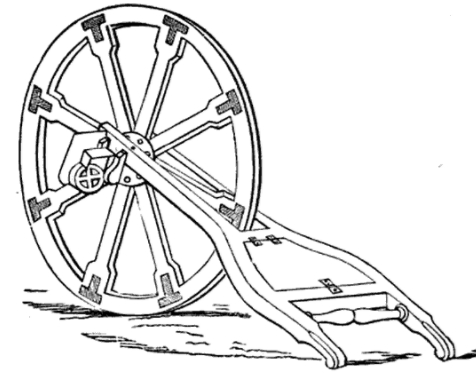
\includegraphics{"images/image008.jpg"}
\caption{ಪೆರಾಂಬ್ಯುಲೇಟರ್​}\label{chap5-fig2}
\end{figure}

ಟ್ರಿಗನಮಿಟ್ರಿಕಲ್​ ಸರ್ವೇ ತಂಡವು ಆರಂಭದ ಲ್ಯಾಂಬಟನ್​ರವರ ದಿನಗಳಲ್ಲಿ ಸರಕು ಹೊರುವ ಕೂಲಿಗಳು, ಕಾರ್ಪೆಂಟರುಗಳು, ನೀರು ಸರಬರಾಜು ಮಾಡುವರು, ಸಂದೇಶ ವಾಹಕರು, ಧೂತರು, ದುಭಾಷಿಗಳು ಇವರಿಂದ ಕೂಡಿರುತ್ತಿತ್ತು. ಇವರ ಜೊತೆಗೆ ಸರಪಳಿ ಎಳೆಯುವರು, ಬಾವುಟ ಹಿಡಿಯುವರು ಇದ್ದೇ ಇರುತಿದ್ದರು. ಮುಂದಿನ ದಿನಗಳಲ್ಲಿ ಜಾರ್ಜ್ ಎವರೆಸ್ಟ್​ರವರು ಟ್ರಿಗನಮಿಟ್ರಿಕಲ್​ ಸರ್ವೇಯ ಮುಖ್ಯಸ್ಥರಾದ ಮೇಲೆ, ಸರ್ವೇ ತಂಡದ ಬಲವು ವೃದ್ಧಿಯಾಯಿತು. ಎವರೆಸ್ಟ್​ರವರ ಸರ್ವೇ ತಂಡದಲ್ಲಿ, ಪ್ರಮುಖರ ಸವಾರಿಗಾಗಿ \enginline{4} ಆನೆಗಳು, ಮಿಲಿಟರಿ ಅಧಿಕಾರಿಗಳ ಪ್ರಯಾಣದ ಅನುಕೂಲಕ್ಕಾಗಿ \enginline{30} ಕುದುರೆಗಳು, ಸರಕು ಸಾಮಾನುಗಳನ್ನು ಹೊರಲು \enginline{42} ಒಂಟೆಗಳು ಇದ್ದವು. ಆಗ ಅದು ಸುಮಾರು \enginline{700} ಜನಬಲ ಇರುವ ಸರ್ವೇ ತಂಡವಾಗಿತ್ತು. ಮುಖ್ಯ ಥಿಯಡೋಲೈಟ್​ನ್ನು ಎತ್ತಿನಗಾಡಿಯ ಕುಲುಕಾಟದ ಕಾರಣದಿಂದ ಗಾಡಿಯಲ್ಲಿ ಸಾಗಿಸದೆ, ಪಳಗಿದ ಕೂಲಿಗಳಿಂದ ಹೊತ್ತು ಸಾಗಿಸಲಾಗುತ್ತಿತ್ತು. ಕಾಡಿನ ಸರ್ವೇ ತಾಣದಲ್ಲಿ, ಅಧಿಕಾರಿಗಳ ವಾಸಕ್ಕೆ ಟೆಂಟ್​ ಇರುತ್ತಿತ್ತು. ಅಧಿಕಾರಿಗಳಿಗೆ ಅದೇ ಆಫೀಸು, ಅದೇ ಮನೆ. ಅವರ ತಂಡದ ಉಳಿದ ಕೆಲಸಗಾರ ಜನಕ್ಕೆ ಟೆಂಟೂ ಇಲ್ಲ, ಯಾವ ಸೂರೂ ಇಲ್ಲ. ಮಳೆಗಾಲದಲ್ಲಿ ಅಕ್ಕ ಪಕ್ಕ ಗುಹೆ ಸಿಕ್ಕರೆ, ಅದೇ ಅವರ ವಾಸದ ಮನೆ. ಬೇಸಿಗೆಯಲ್ಲಿ ಮರದ ಕೆಳಗಿನ ಬಯಲೇ ಗತಿ. ಇವರೆಲ್ಲರೂ ಬಲು ಕಠಿಣ ಪರಿಸರದಲ್ಲಿ, ಬಹು ಎಚ್ಚರಿಕೆಯಿಂದ, ಕರಾರುವಕ್ಕಾಗಿ ನಡೆಸಿದ ಈ ಸರ್ವೇಯ ಕಾರ್ಯದಲ್ಲಿ ತಮ್ಮದೇ ಆದ ತ್ಯಾಗವನ್ನು ಮಾಡಿದ್ದಾರೆ.

\begin{figure}[!htbp]
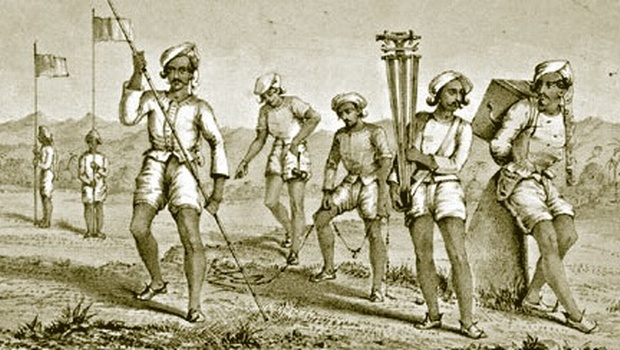
\includegraphics{"images/image009.jpg"}
\caption{ಸರ್ವೆ ತಂಡದ ಕೆಲಸಗಾರರು (ಕೃಪೆ: ವಿಕಿಪಿಡಿಯಾ)}\label{chap5-fig3}
\end{figure}

